\documentclass[12pt,a4paper]{article}
\usepackage[a4paper, margin=1.5cm]{geometry}
\usepackage{graphicx}
\graphicspath{{./images/}}
\usepackage{subcaption}
\newcommand{\tr}{\mathrm{tr}}
\usepackage{hyperref}
\usepackage{authblk}
\usepackage[backend=biber,style=nature]{biblatex}

\bibliography{article}
\addbibresource{article.bib}


\begin{document}
\title{Ionizations of Liquid Water from Charged-cell Periodic Subsystem DFT and Embedded Coupled Cluster Simulations}
\author[1]{Jessica Martinez}
\author[1]{Pablo Ramos}
\affil[1]{Department of Chemistry, Rutgers University, Newark, New Jersey}
\author[2]{Andre Gomes}
\affil[2]{Université de Lille, CNRS, UMR 8523 – PhLAM – Physique des Lasers, Atomes et Molécules, Lille, France}
\author[3]{Johannes Tölle}
\affil[3]{Theoretische Organische Chemie, OrganischChemisches Institut and Center for Multiscale Theory and Computation (CMTC), Westfälische Wilhelms-Universität Münster, Corrensstraße 40, 48149, Münster, Germany}
\author[1]{Michele Pavanello}
\date{}
\setcounter{Maxaffil}{0}
\renewcommand\Affilfont{\itshape\small}
\begin{titlepage}
  \maketitle
\end{titlepage}

\begin{abstract}
Modeling the ionization potential (IP) and electron affinity (EA) of liquid water is challenging for
two reasons: (1) the bulk-like nature of the liquid imposes the use of periodic boundary conditions
(PBCs), which pose roadblocks when considering charge systems; (2) quantitative electronic structure
methods, such as coupled cluster, are generally not available in PBCs. In this work, we tackle both
challenges by employing subsystem DFT to split the extended system into a collection of finite
subsystems embedded by extended, infinite subsystem. This is achieved by an impurity
model ~\cite{tolle2019charged} where high ab initio method as coupled cluster wavefunctions can be introduced to evaluate
the water molecules’ energy functionals. 

The liquid’s electronic structure is expressed in subsystem contributions by invoking nonadditive density 
functionals whereby the total energy of the liquid is expressed as the sum of molecule-additive
and nonadditive contributions ~\cite{krishtal2015subsystem}. The inter-molecular interaction is
split into Coulumb interactions, and such nonadditive terms as the noninteracting
kinetic energy and the noninteracting exchange-correlation ~\cite{krishtal2015subsystem}. 
These contributions represent interactions related among others to exchange, van der Waals and
Pauli repulsion and are all bifunctional of the subsystem densities ~\cite{tolle2019charged}. 

The final IP/EA values reproduce the experimental values to within 0.5 eV and are determined averaging 
over 256 water molecules (or subsystems) considered in the simulation cell, calculated by the energy difference of the
neutral and the polarized system (Called SCF method) ~\cite{bagus1965self,waskom2017mwaskom}. 
\end{abstract}


\section{Introduction}

The high-accuracy calculations of ionization potentials (IPs) and electron affinities (EAs) of condensed-phase molecular systems as liquid water has 
represented a challege for the last years in both experimental and computational fields \cite{tolle2019charged,gaiduk2018electron,gaiduk2016photoelectron,seidel2016valence}. Thus, ionized states of the electrons take part in many crucial processes in electrochemistry, photochemistry as well as
exotic states of matter as the solvated electron \cite{ambrosio2017electronic}. The most recent theoretical report of IP and EA values
\cite{ziaei2018probing} shows that using quasi-particle self-consistent GW calculations and implicit vertex correction in many-body perturbation
(MBPT) considerably affect the EA previous reported \cite{gaiduk2018electron} by about 1eV. Therefore, trough self-consistent GW approach with an
implicit vertex correction based on the projector augmented wave (PAW) method, which is the most accurate pseudo-potential (PPs available),
and combined with Bethe–Salpeter equation establish values of 10.2 and 1.1 eV, for IP and EA of liquid water, respectively.

Following the trend and now including the use of periodic boundary conditions (PBC) another method was introduced \cite{tolle2019charged}
to determine the ionization potentials (IPs) and electron affinities (EAs) of liquid water. Based on determining successfully a quatum-mechanical
models for charged species in PBC which is able to face the complications related to the long-ranged nature of the Coulomb Kernel
$ w(r,r^{'}) = \frac {1}{|r - r^{'}|}$, which decays to zero when two charges are far away. Indeed, it is precisely what previous research achieved
using an impurity model with two remarkable qualities: 1) The charged periodic system is replaced by a non-periodic one which is still truly
extended (ie., of infinite size) and 2) The potentials of the neutral and the charged system are pegged to a common reference. 

Achieving the former requires an ad hoc mapping of the infinite system(periodic) onto finite number of finite subsystems
(non-periodic subsystems) and an extended (infinite) subsystem, using a formally exact density embedding method, subsystem DFT. Meanwhile, achieving
the latter only requires finding a consistent choice for the $G = 0$ component of the Coulomb Kernel in a reciprocal space. The above is possible due
to the total charged density $\rho (G)$ is zero, although the kernel singularity for $w(G)$ at $G = 0$.

\section{Theoretical Background}

\subsection{Mapping a periodic system into a collection of non-periodic subsystems and one periodic subsystem}

To cast DFT in a subsystem fashion, we invoke nonadditive functionals in which each energy term of the supersystem is expressed as the sum of additive
and nonadditive contributions ~\cite{martyna1999reciprocal}. Therefore, when dealing with a finite subsystem with electron density $\eta_I$, and an
infinite or extended subsystem with electron density $\eta$ - $\eta_I$, the total energy is given by,

\begin{equation}
	E_{tot} = {E_[{\eta}_I]} + {E_[{\eta} - {\eta}_I]} + {E^{int}[{\eta}_I, {\eta} - {\eta}_I] } 
\end{equation}

And the interaction energy can be broken down into the following contributions,

\begin{equation}
	E^{int} = E^{int}_H + V^{int}_eN + T^{nad}_s + E^{nad}_{xc} 
\end{equation}

The two Coulombic terms $E^{int}_H$ and $V^{int}_eN$ are the electron-electron and electro-nuclear interactions, respectively. And the
nonadditive terms $T^{nad}_s$ and $E^{nad}_{xc}$, represent the noninteracting kinetic energy of the system and the noninteracting
exchange-correlation functionals, respectively ~\cite{krishtal2015subsystem}. The two last terms represent interactions related among other to exchange, van der Waals and Pauli repulsion and are all bifunctional of the two subsystem densities.

\subsection{Coulomb interaction energy determination}



\subsection{Embedding Scheme for the Neutral System}

For the neutral system, the Coulomb interaction energy can be expressed as a potential that maps the interaction of an accurately infinitely extended
environment onto and isolated subsystem $I$,

\begin{equation}
	v^{'}_{int} [\eta] (r) = v[\eta](r) - \bar{v} [\eta_I](r)
\end{equation}

Where $v[\eta](r)$ is the total Coulomb potential of the system and $\bar{v} [\eta_I](r)$ the potential of the isolated subsystem $I$. The latter was
evaluated using the Martyna-Tuckerman method whereby density $\eta_I$ is assumed to be isolated and not periodic \cite{martyna1999reciprocal}.
The embedding potential for the neutral subsystem can also be calculated directly from equation $3$.

\subsection{Impurity Model for the Ionized system}

To obtain the embedding potential of a charged subsystem, we consider the system to be composed of an ionized subsystem embedded in a nonionized
environment. To assemble the appropriate embedding potential, first was evaluated a screening potential,
$v^{screen}[\eta_I](r) = v[\eta_I](r) - \bar{v} [\eta_I](r)$, for both charged and neutral subsystems (understood as a self-interaction of the
charge in PBC). The embedding potential depends on thre densities: $\eta$, the total system, $\eta^{'}_I$, the neutral subsystem, and $\eta_I$ the
charged subsystem, and has the form,

\begin{equation}
	v^I_{emb,imp}[\eta](r) = v[\eta, \eta^{'}_I, \eta_I](r) - \bar{\eta_I}(r)
\end{equation}

with

\begin{equation}
	v[\eta, \eta^{'}_I, \eta_I](r) = v[\eta](r) + \Delta{v}^{screen}[\eta_I, \eta^{'}_I](r)
\end{equation}

where $\Delta{v}^{screen}[\eta_I, \eta^{'}_I](r) = {v}^{screen}[\eta^{'}_I] - {v}^{screen}[\eta_I]$

\section{Computational Section}

All calculatons were carried out with embedded Quatum ESPRESSO (eEQ) employing ultrasoft pseudopotentials. The graound state calculation of each
subsystem with the corresponding neutral and polarized embedding potential was determined through ADF \cite{te2001chemistry} software. A comparison
among Density Functional Theory (DFT), using GGA(PBE), Hybrid(B3LYP), Double-Hybrid (B2KPLYP, B2NCPLYP, and REVDSDBLYP) and Statistical average of
orbital potentials(SOAP) models, Møller–Plesset perturbation theory (MP2) and HF methods was made, with the basis QZ4P. The final IP/EA values are
calculated using an average for each of the 256 water molecules or subsystems considered in the simulation cell, calculated by the energy difference
of the neutral and the polarized system (Called $\Delta$SCF method) \cite{bagus1965self,waskom2017mwaskom}.

\section{Results}
\subsection{IPs of Bulk water}

\begin{figure}[!h]
	\captionsetup[subfigure]{labelformat=empty}
	\centering
	\begin{subfigure}{0.4\linewidth}
		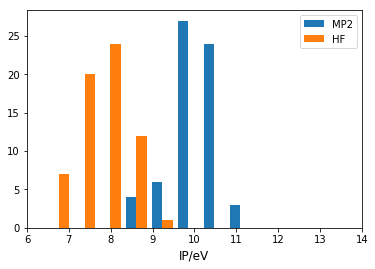
\includegraphics[width=\linewidth]{IP-mp2-hf}
		\caption{MP2 vs HF}
	\end{subfigure}
	\begin{subfigure}{0.4\linewidth}
		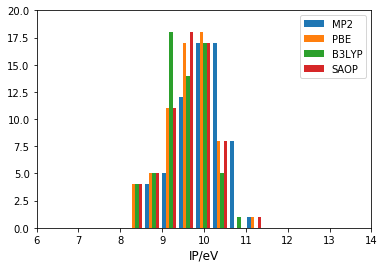
\includegraphics[width=\linewidth]{IP-mp2-dft}
		\caption{MP2 vs DFT}
	\end{subfigure}
	\caption{Distribution of IPs of bulk liquid water. The area subtenended by the lines sums up to 64(ie, the number of subsystems). Left: Comparison between MP2 and HF. Right: Comparison between MP2 and DFT}
\end{figure}

\begin{table}[!h]
 \begin{center}
  \caption{average IPs}
  \label{tab:table1}
  \begin{tabular}{ |c|c| }
	\hline\hline
	&IP average (eV)\\
	\hline
	MP2&9.9941\\
	\hline
	HF& 7.8250\\
	\hline
	PBE&9.6089\\
        \hline
        B3LYP&9.5147\\
        \hline
        SAOP&9.5897\\
	\hline
   \end{tabular}
 \end{center}
\end{table}

\section{Conclusions}

\nocite{*}

\printbibliography

\section{Acknowledgments}


\end{document}
